\chapter{TuMag's design and calibration.}

In this chapter we take the first steps of the journey of developing an instrument to observe the Sun. We will define... 

Fabry-Pérot interferometers (FPIs) are widely employed in the field of solar physics. Their spectroscopic and tunability properties make them especially suitable for selecting a narrow spectral band of incoming light. They also offer a two-dimensional view of the solar scene, hence allowing for the implementation of powerful and widespread image post-processing reconstruction techniques, such as phase diversity \citep{PD_etalon} and multi-object multi-frame blind deconvolution (MOMFBD; \citealt{mombfd}), which are difficult to implement in slit-based spectrographs (\citealt{image_spectro}, \citealt{image_spectro_2}). Many state-of-the-art instruments use FPIs as narrowband tunable filters. Among others, these instruments include the spaceborne Polarimetric and Helioseismic Imager \citep[][]{PHI} aboard the Solar Orbiter mission \citep[][]{SO} (SO/PHI); the Imaging Magnetograph Experiment (IMaX) instrument \citep[][]{IMaX}, which flew on the first two flights of the balloon-born SUNRISE observatory (\citealt{SunriseI}, \citealt{SunriseII}); and the Tunable Magnetograph (TuMag) instrument for its third edition. These instruments are based on solid LiNbO$_3$ etalons. Regarding ground-based instruments, some examples include the Crisp Imaging Spectro-Polarimeter (CRISP) at the Swedish 1-m Solar telescope \citep[][]{crisp} at the Observatorio del Roque de los Muchachos in La Palma, Canary Islands; the GREGOR Fabry-Perot Interferometer (GFPI; \citealt{GFPI}, \citealt{GREGOR}) at the Observatorio del Teide in Tenerife, Canary Islands; the Visible Tunable Filter \citep[VTF;][]{VTF} developed for the \textit{Daniel K. Inouye} Solar Telescope \citep[DKIST;][]{DKIST} of the Haleakal\=a Observatory in Hawaii; and the future Tunable Imaging Spectropolarimeter (TIS) of the European Solar Telescope \citep{EST}, all of which are based on air-gapped etalons. 




The SUNRISE III mission aims to study and stablish the relations and couplings between the phenomena ocurring at different layers of the Sun's surface. With this purpose in mind, three different post-focal instruments were included in the design, each of them responsible of observing at different regions of the spectrum. The SUNRISE UV Spectropolarimeter and Imager (SUSI, \textbf{REFERENCIA}), which will observe the spectra between 309 nm and 417 nm; The Sunrise Chromospheric Infrared spectroPolarimeter (SCIP, \textbf{REFERENCIA}), which will observe the near-infrared; and lastly, the Tunable Magnetograph (TuMag), which will observe three spectral lines in the visible, at 525.02 nm, 525.06 nm and 517 nm. 

The design from scratch of an instrument such as this is very complex. There are many things that have to be meticulously designed and tested which span many fields of expertise, like optics, electronics, software, hardware, or thermal design. To avoid undue extension of this thesis, we will focus on the aspects of the design directly related to the \textbf{TO QUE}, that is, regarding the spectral, imaging and polarimetric capabilities of the instrument. 

\section{A brief introduction to spectropolarimeters.}

Spectropolarimeters, as suggested by the name, are devices that measure the spectral and polarimetric properties of light, or in other words, that measure the polarization state of light as a function of wavelength. Their use is widely extended in astrophysics due to the huge amout of information about the light source we can infer from these properties.

In solar physics, it is common to encounter two distinct types of spectropolarimeters, distinguished by their approach to spectroscopy: slit-based spectrographs, such as SUSI and SCIP, and narrow-band tunable filtergraphs, like TuMag. The latter preserve spatial resolution by capturing two-dimensional images of the solar scene at the expense of sacrificing spectral resolution. Conversely, slit-based spectrographs provide excellent spectral resolution but have a limited spatial resolution. 

Regardless of how spectroscopy is carried out, spectropolarimeters must be able to measure the polarization state of light. That is, they must be capable of determining the Stokes parameters  of the incident light. These four parameters, usually grouped in a pseudo-vector: $[I, Q, U, V]$, were defined by Stokes in \cite{Stokes_vector} as a mathematical formalism to completely define to polarization state of light. The first parameter, $I$, represents the total intensity; $Q$ and $U$ provide information about the intensity of linearly-polarized light, at 0º and 90º, respectively; and lastly, $V$, accounts for the intensity of circularly polarized light. 

Excellent polarimetric sensitivity and spectral resolution are wasted if the optical capabilities of the instrument are not up to par. The design of these instruments must achieve diffraction-limited imaging, with a signal-to-noise ratio ensuring a polarimetric sensitivity of 1000 (typically), and the best spatial resolution the telescope allows, all without sacrificing spectral resolution and accomplishing this in the shortest possible time.

When designing the instrument, one must balance these three properties: spectral, optical, and polarimetric capabilities, trying to improve the performance in all of them without sacrificing too much. In the following sections, we will delve into each of these aspects in more detail.

\subsection{Spectroscopy}

Narrow-band tunable spectrographs play a significant role in this thesis. They will be extensively discussed in this chapter, particularly in relation to the design and calibration of TuMag, and again in Chapters \ref{CH:Pipeline} and \ref{CH:challenges} when addressing TuMag's pipeline and the correction of data produced by these instruments. Therefore, for the sake of simplicity, we will focus exclusively on this type of spectrographs from this point onward.

\textcolor{red}{CAMBIAR ESTO}.

Fabry-Pérot Interferometers (FPIs), also known as etalons (used interchangeably), represent one of the most prevalent forms of narrow-band tunable spectrographs. Composed by a resonant optical cavity formed by two distinct optical media, these devices allow only the passage of light with wavelengths corresponding to constructive interference within the cavity. 

The transmission profile of an etalon, being produced by an interference phenomenon, is characterized by a series of narrow and periodic transmission peaks. The wavelengths at which this resonance peaks are located, their width, and their separation are determined solely by the physical properties of the etalon. In fact, it is not difficult to demonstrate \citep{franI} that a resonant cavity produces a periodic transmission profile, with maxima occurring at a wavelength $\lambda$ such that:

\textcolor{red}{REVISAR -> VÁLIDO PARA TELECENTRIC??} 

\begin{equation}
\lambda = \frac{2nd\cos \theta}{m}\ ,
\label{eq_ch2: order_sorting}
\end{equation}
where $n$ is the refractive index of the medium inside the cavity, $d$ is the distance between the mirrors, $\theta$ is the angle of incidence of the incoming light ray and m is the interferential order ($m \in \mathbb{Z} $). 

With Eq.~\eqref{eq_ch2: order_sorting} in mind, it is clear that an etalon allows for tuning the wavelengths of the transmission peaks by either changing the distance between the mirrors or by altering the refractive index. Although changing the angle of incidence also results in a wavelength shift, it introduces other issues, such as ghost images or profile broadening in telecentric configurations, among other effects. Consequently, the angle is not used for wavelength tuning.

To tune to a single wavelength (or a very narrow band around it), it is necessary to isolate one transmission peak (main order). This is typically achieved by using a pre-filter that only allows light with wavelengths near the desired measurement region to pass through. This ensures that no light reaches the etalon that could pass through it due to interference orders other than the main one (secondary orders). 

\begin{figure}
  \centering
  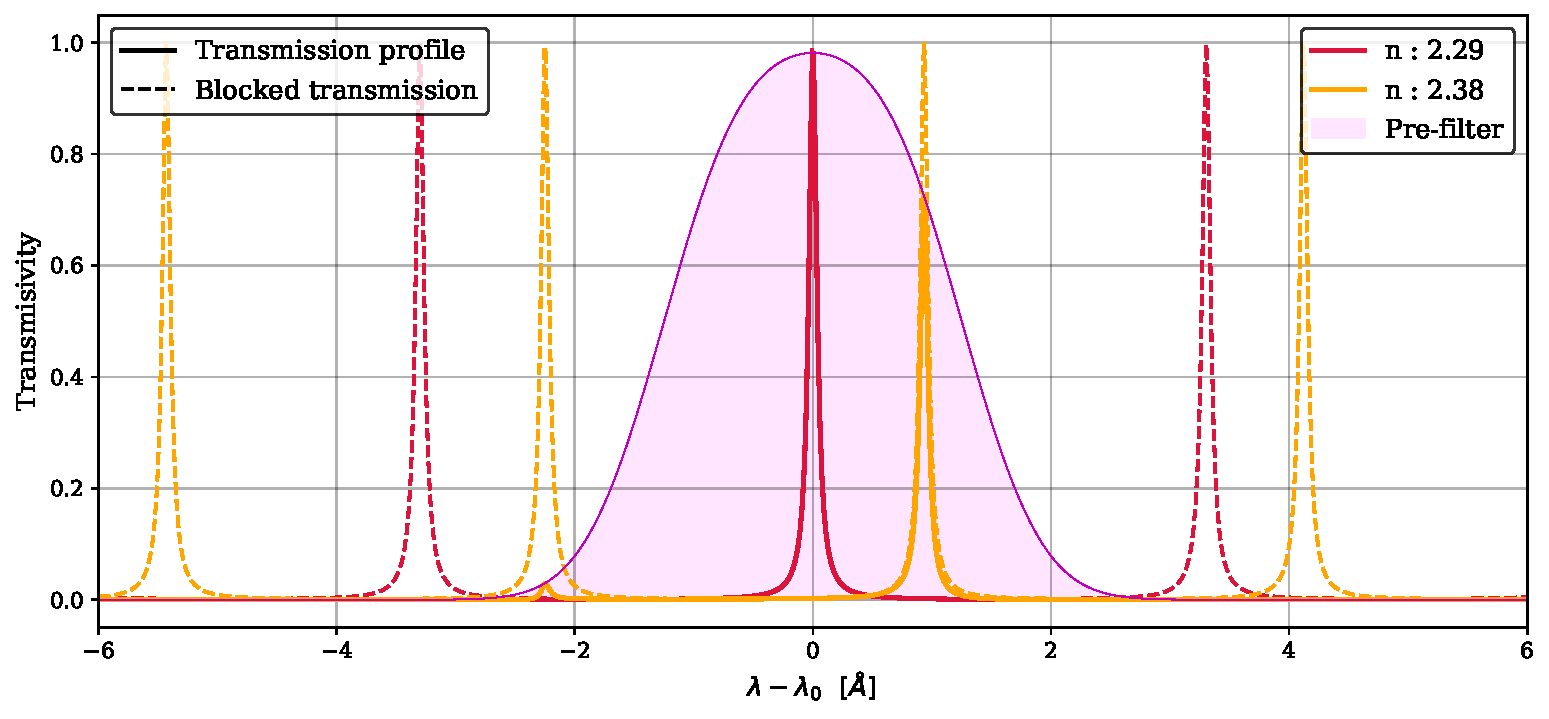
\includegraphics[width = \textwidth]{figures/Introduction_to_spectropolarimeters/Etalon_and_prefilter_example.pdf}
  \caption{Transmission profiles of the same etalon with varying refractive indices (n). The dashed lines represent the original transmission profile, while the solid lines indicate the portion of the transmission profile that passes through the order-sorting pre-filter (shaded purple area).} 
  \label{fig_ch2: etalon_example}
\end{figure}

Figure \ref{fig_ch2: etalon_example} shows a simulation of the spectral behavior of this optical setup. The order-sorting pre-filter is shown with a shaded purple area and the unaltered transmission profile of the etalon is shown in dahsed lines for different values of the refractive index. In solid lines, the resulting transmission profile is shown, that is, the transmission allowed through both the pre-filter and etalon at the same time. 

\subsection{Polarimetry}

\textcolor{red}{As previously noted, determining the polarization state of light requires the determination of the components of the Stokes vector. However, these parameters cannot be measured directly since we only know how to measure intensities. Since they are  Thus, measuring the polarization of light always involves multiple measurements at once. Specifically, a number equal to the number of elements to be determineed: four for the complete Stokes vector, or two, if only the circular polarization and total intensity are to be measured. This is the root of the difficulties in measuring polarization, as the need for multiple measurements makes them much more susceptible to spurious effects compared to individual measurements.} Cambiar que es un jaleo. 

Mathematically, the effect on polarization of a linear and finite system can be treated as a combination of linear transformations on the Stokes vector and, therefore, can be represented by a matrix in $\mathbb{R}^4$, known as the \textit{Mueller Matrix}. Let $\textbf{M}$ be the matrix that describes these transformations, then the polarization state that reaches the detector follows:

\begin{equation}
  \textbf{I}_{out} = \textbf{M}\textbf{I}_{in},
\end{equation}
where $\textbf{I}_{in}$ and $\textbf{I}_{out}$ are the Stokes vectors of the light that reaches the instrument, and the detector, respectively. However, since we only know how to measure intensities, the actual quantity measured by our CCD is: 

\begin{equation}
  I_{obs} = m_{00}I_{in} + m_{01}Q_{in} + m_{02}U_{in} + m_{03}V_{in} \ \ ,
\end{equation}
where $m_{0i}$ is the i-th element of the first row of the Mueller Matrix. This means that the intensity we measure is a linear combination of the different polarization states of the incoming light. To determine the values of the individual parameters $I_{in}$, $Q_{in}$, $U_{in}$, and $V_{in}$, further independent measurements are necessary, which can be achieved by modifying the Mueller matrix. In particular, it is easy to see that four independent measurements are required in order to construct a system of equations that allows us to determine the full Stokes vector. This process is known as modulation, and the four independent measurements are referred to as modulations.

If we denote each of the modulations by $I _ j$ with $j \in \left\{ 1, 2, 3, 4\right\}$, we can construct the following system of equations:

\begin{equation}
  \begin{pmatrix}
  I _ 1 \\
  I _ 2 \\
  I _ 3 \\
  I _ 4
  \end{pmatrix} = 
  \underbrace{\begin{pmatrix} 
      m ^ 1 _ {01} & m ^ 1 _ {02} & m ^ 1 _ {03} & m ^ 1 _ {04} \\ 
      m ^ 2 _ {01} & m ^ 2 _ {02} & m ^ 2 _ {03} & m ^ 2 _ {04} \\
      m ^ 3 _ {01} & m ^ 3 _ {02} & m ^ 3 _ {03} & m ^ 3 _ {04} \\
      m ^ 4 _ {01} & m ^ 4 _ {02} & m ^ 4 _ {03} & m ^ 4 _ {04} 
  \end{pmatrix}}_ {\textbf{O}}
  \begin{pmatrix}
    I _ {in} \\
    U _ {in} \\
    Q _ {in} \\
    V _ {in}
    \end{pmatrix} \, 
    \label{eq_spectro_theory: stokes_linear_comb}
\end{equation}
where the superindex in $m ^j _{oi}$ denotes the values of the Mueller Matrix for each modulation. Through straightforward algebra, it is easy to see that the stokes vector of the incoming light can be determined by $\textbf{I}_{in} = \textbf{D}\textbf{I}_{obs}$, where $\textbf{D}$ is the demodulation matrix, the inverse of the modulation matrix, $\textbf{O}$, and $\textbf{I}_{obs}$ is the vector containing the 4 measured modulations. Accurately determining $\textbf{O}$ during the instrument calibration process is crucial, as the determination of the Stokes components depends entirely upon it.

\subsection{\label{susec_spectropolarimeters: Imaging}Imaging}

\textcolor{red}{The high-resolution imaging that etalon-based instruments are capable of is one of the pivotal reasons for their extended use. The ability to capture a two-dimensional scene of the solar surface makes them ideal for studying solar plasma structures, which require resolutions close to 100 km on the solar surface. However, it is essential to achieve these resolutions while maintaining a sufficiently high signal-to-noise ratio to ensure the required polarimetric sensitivity.}

Spectropolarimeters ultimately combine measurements in polarization, spectral, and spatial (image) domains. Consequently, the final observed intensity depends on all three properties simultaneously. By integrating the spectral behavior of the etalon and pre-filter with the polatrimetric measurements, and taking into account the spatial dependence of these measurements, the observed intensity for a modulation $j$ at any point of the focal plane $\eta, \xi$ when the etalon is tuned at a wavelength $\lambda _ s$ is determined by:

\begin{equation}
  I_ j\left(\xi, \eta ; \lambda_{s}\right)=g(\xi, \eta)\int_{0}^{\infty} T(\lambda) \iint  O _ j\left(\xi_0, \eta_0 ; \lambda\right)  \mathcal{S}\left(\xi_0, \eta_0; \xi , \eta; \lambda-\lambda_{s}\right)  \mathrm{d} \xi_{0} \mathrm{~d} \eta_{0}\mathrm{d} \lambda ,
  \label{eq_spectro: General_Intensity}
\end{equation}
where $T(\lambda)$ accounts for the presence of the order-sorting pre-filter, $S\left(\xi_0, \eta_0; \xi , \eta; \lambda-\lambda_{s}\right)$ accounts for the imaging response of the instrument when tuned at the wavelength $\lambda_{s}$, $g(\xi, \eta)$ represents a spatial gain factor that accounts for any wavelength independent pixel-to-pixel intensity fluctuations ocurring in the focal plane, and $O _ j(\xi_0, \eta_ 0;\lambda)$ is the intensity distribution of the incoming light for a modulation j and is given by:
\begin{equation}
  O _ j(\xi_0, \eta_ 0;\lambda) = m_{00} ^jI_{in}(\xi_0, \eta_ 0;\lambda) + m_{01}^jQ_{in}(\xi_0, \eta_ 0;\lambda) + m_{02}^jU_{in}(\xi_0, \eta_ 0;\lambda) + m_{03}^jV_{in}(\xi_0, \eta_ 0;\lambda)
\end{equation}

Determining the imaging response of the instrument can be quite complex , as it is influenced not only by their physical characteristics but also by their optical configuration, whether collimated or telecentric. In Chapter 2, we provide a detailed overview of the properties of each configuration, their differences, and the challenges involved in using these devices for data correction.

\textcolor{red}{ADD noise Discussion?}
 
\subsection{What do spectrpolarimeters tell us about the Sun?}

Spectropolarimeters are often referred to as magnetographs (\textit{e.g.}, TuMag), suggesting they measure magnetic fields directly. However, this is not entirely accurate. In astrophysics, the physical properties of the light source are inferred by correlating them with the observed properties of the light, rather than measuring them directly. By evaluating the polarization of sunlight at different wavelengths, spectropolarimeters enable us to infer the magnetic field and estimate plasma velocities on the solar surface. 

The simplest calculation we can carry out that provides us with physical quantities of the Sun is that of the line-of-sight (LOS) velocities. Given the spectral shift of a specific absorption or emission spectral line, $\Delta \lambda$, with respect to its rest position, $\lambda _ 0$ , the LOS velocities can be computed with the Doppler formula: 
\begin{equation}
  v_{LOS} = \frac{\Delta \lambda}{\lambda _ 0}c\ \ ,
  \label{eq_spectro: Doppler}
\end{equation}
where $c$ stands for the speed of light in vacuum. 

The polarization properties of light come into play when determining the magnetic fields. Due to Zeeman and Hanle effects, the polarity and spetcroscopy of spectral lines can be altered when formed in the presence of magnetic fields. Due to the Zeeman effect, the spectral lines widen or split into different polarized components when a strong magnetic field is present \citep{libro_JoseCarlos}, such as in the surroundings of sunspots and active regions. In the other hand, the Hanle effect is sensitive to weaker fields, and can be used to study the magnetic structure of solar prominences or turbulent fields in the solar photosphere \citep{hanle}. 

One simple strategy to employ polarization and spectral data to derive the magnetic fields is through the center-of-gravity method. According to \cite{center_of_gravity}, the LOS strength of the magnetic field can be obtained through:
\begin{equation}
  B_{LOS} = \frac{\lambda _ {+} - \lambda _ -}{2}\frac{4\pi m c}{eg_{L}\lambda_0 ^2}\ \ ,
  \label{eq_spectro: Blos-cog}
\end{equation}  
where $m$ and $e$ are the electron mass and charge respectively, $g_L$ stands for the Landé factor and $\lambda _ {+}$ and $\lambda _ {-}$ are the centroids of the right and left circularly polarized line components, respectively, and are computed by:
\begin{equation}
  \lambda _ {\pm} = \frac{\int \lambda \left[I_{cont} - (I \pm V)\right]d\lambda}{\int \left[I_{cont} - (I \pm V)\right]d\lambda} \ ,
  \label{eq_spectro: lambda_plus_minus}
\end{equation} 

where the subindex "$cont$" stands for the wavelength at the continuum. 

The vector magnetic field (\textit{i.e.}, strength, azimuth and inclination), and not only the LOS strength can also be derived. However, the derivation of these quantities has to be achieved through inversions of the radiative transfer equation (RTE). The applicability of the different methods to carry out this inversion is an extensive topic as there are some assumptions that can be applied in some cases but not in others, such as the weak-field or Milne-Eddington approximations, among others. For an extended discussion of this topic, we refer the interested reader to \cite{del2016inversion}.   

\section{The Tunable magnetograph: TuMag}

Among many examples of spectropolarimeters, one that has special relevance for this thesis is TuMag. The Tunable magnetograph (TuMag) is a wavelength-tunable spectropolarimeter that observes in the photosphere and the low chromosphere. 

TuMag is a filtergraph that employs a solid LiNbO$_3$-based FPI to scan the spectral lines. This kind of etalons are able to change the refractive index of the matierial inside the cavity by applying a voltage difference between the two mirrors. This design advantageously eliminates moving parts from the tuning process, though it requires high voltages for operation. 

In order to be able to carry out observations of both the photosphere and low cromosphere, TuMag must be able to switch between different spectral lines. For this purpose, TuMag is equipped with three different pre-filters centered at the wavelengths of three different spectral lines: The FeI line at $5250.2$ \r{A}, the FeI line at $5250.6$ \r{A}, and the Mg line at $5172.7$ \r{A}.  


\section{Calibration of TuMag}